\section{\label{sec:cable}Cable Systems}

The IceCube detector may be viewed as a digital network of optical
sensors. The IceCube cable systems form the physical backbone of this
network, simultaneously supplying power to the DOMs and bi-directional
digital communications between the DOMs and the readout hardware at the
surface. Due to a previous successful demonstration of the
digital-readout optical modules contained within the AMANDA detector
\cite{AMANDA:string18} and concerns with mechanical robustness of
optical fiber during
freeze-in in the deep ice, copper was chosen over fiber at an early stage in the
project.

\subsection{Design}

The cable system comprises the following assemblies: the in-ice cable,
IceTop cables, the surface junction box (SJB), the surface cables, and the patch
cables. The in-ice cable, 2505~m long, is deployed
into the ice along with 60 DOMs that are attached to connectors at 30
breakouts spaced 34~m apart. Each pair of DOMs is connected to a unique
single twisted wire pair. Wire pairs are combined into four-conductor quad
cables meeting stringent electrical performance requirements. The 60
DOMs on each cable require 15 quads. An additional 5 quads in the
in-ice cable provide for special instrumentation connections, a spare quad,
and local coincidence connections between adjacent DOMs. The in-ice
cable terminates at the SJB, located just below the snow surface between
the IceTop tanks. The SJB is a stainless steel
enclosure that houses the in-ice cable and surface cable
connections. IceTop cables also terminate and connect to the surface cable
in the SJB. The surface cable is trenched 1~m deep into the
surface of the snow between the SJB and the ICL. The surface
cables vary in length from 300~m to approximately 800~m in length depending on hole location. The surface cables are
pulled up two cable towers into the ICL and terminate at patch panels where the individual
quads are separated and connected to patch cables that finally
terminate at the DOMHub, the computer which receives DOM signals in the ICL (see Sec.~\ref{sect:sps}). Each
DOMHub services a single in-ice string or 8 IceTop stations (see
Fig.~\ref{fig:icecube-cables-logical}). IceTop DOMHubs service fewer
DOMs than in-ice DOMHubs due to the higher rates recorded by IceTop DOMs~\cite{ICECUBE:IceTop}.

\begin{figure}
  \centering
  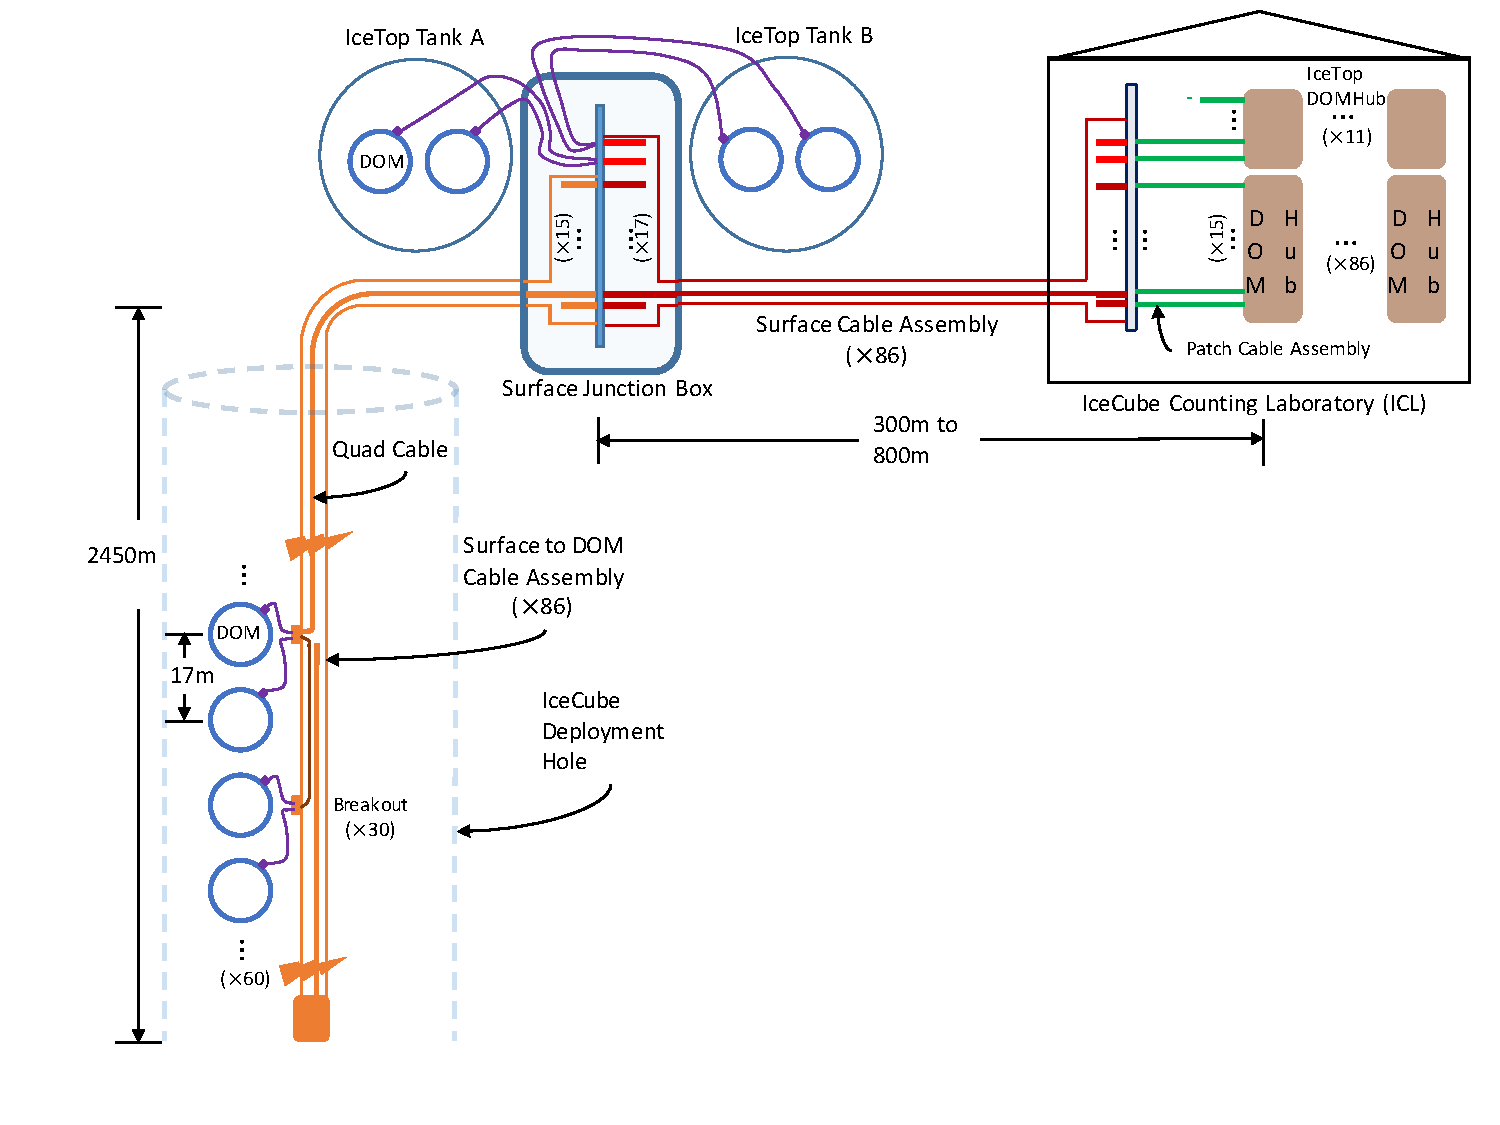
\includegraphics[width=\textwidth]{graphics/cables/cable_system_schematic.pdf}
  \caption{\label{fig:icecube-cables-logical}Schematic of the IceCube cable network architecture.}
\end{figure}

The IceCube cable system design had to meet a technically challenging
variety of mechanical, electrical and functional requirements, under the extreme
conditions of installation at the South Pole, in order for
IceCube to meet its science objectives.  In particular, the in-ice cable
was required to withstand hydrostatic overpressure of up to 450~bar during
deployment.  Handling temperatures were specified down to $-40$~C for all 
cable components.  The primary electrical requirements for the quad
cables are provided in Table ~\ref{tab:quad_requirements}.

% FIX ME CLEAN UP TABLE
\begin{table}[h]
  \centering
  \caption{Electrical requirements for the cable quads.} 
  \begin{tabularx}{\textwidth}{ l X  X  }
    \toprule
    Characteristic& Specification & Conditions \\
    \midrule

    Attenuation & 20 dB maximum & At 1.0 MHz end-to-end \\
   % \hline
%
 %   crosstalk attenuation & intra-quad \& quad-quad & \\
  %  \hline

   Near-end Crosstalk suppression& 50 dB minimum & At 2~MHz \\
(intra-quad and quad-quad)&24 dB minimum& At 100 MHz\\
%\hline
   Far-end Crosstalk suppression& 30 dB minimum & At 2 MHz \\
(intra-quad and quad-quad)&24 dB minimum& At 20 MHz\\

   % \hline

    Differential Impedance & Nominal $145\Omega \pm 10\Omega$ & At 1.0 MHz \\
    %\hline

    Loop Resistance & $160~\Omega$ maximum & \\
    %\hline

    Dielectric breakdown & 2000~VDC minimum, 1.0~$\mu A$ maximum leakage, 60~second
    maximum duration & \\
    \bottomrule  
  \end{tabularx}
  \label{tab:quad_requirements}
\end{table}

 The in-ice cable was also required to be less than 50~mm in
 diameter, weigh less than 2~kg / m, have a minimum static bend radius of 40~cm,
 carry a maximum static tensile load of 10~kN, and have a breaking strength
 of 40~kN.
 
\begin{figure}
  \centering
  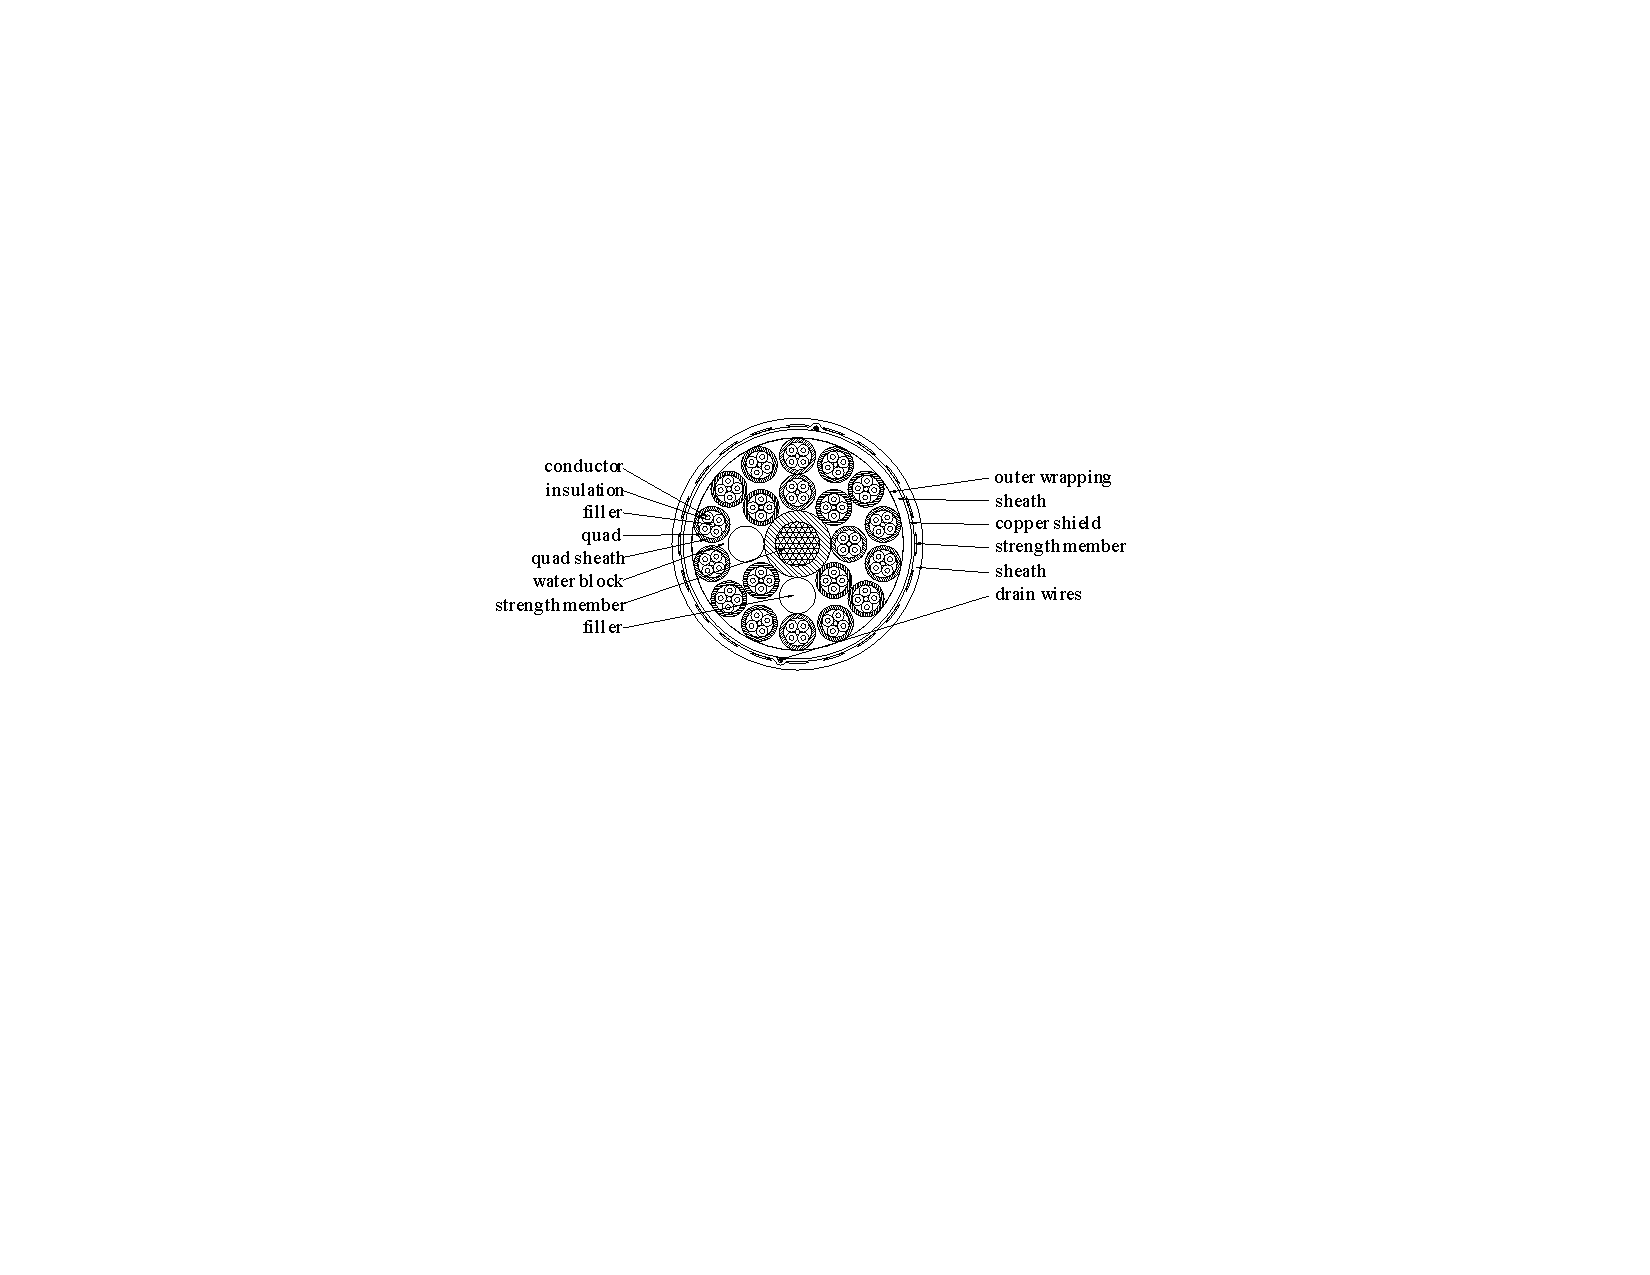
\includegraphics[width=0.5\textwidth]{graphics/cables/labeled_inice_xsection.pdf}
  \caption{\label{fig:cable_xsection}In-ice cable cross
    section, with a nominal 46mm diameter and mass of 2 kg/m.} 
\end{figure}

The in-ice cable includes 20 quads, 2 polyethylene fillers to maintain structural
symmetry, Kevlar outer and inner core strength members, a copper foil
shield with drain wires to provide electrical noise isolation, and a water
block that prevented water or ice from damaging the symmetry of the
cable (see Fig.~\ref{fig:cable_xsection}). The surface cable has a similar
construction to the in-ice 
cable with two exceptions: first, the inner Kevlar strength member was replaced
with additional conductors needed to service the IceTop tanks; and second, the
water block was not required.

A competitive proposal process resulted in two main suppliers for the IceCube
cable system.  Ericsson Network Technologies (Hudiksvall, Sweden) was chosen
to produce the raw cable, and SEACON Brantner \& Associates Inc. (El Cajon,
California) was chosen to manufacture the cable assemblies. The raw
cable was manufactured and tested to meet all required specifications prior to spooling.  The in-ice cables were then
wound onto custom metal spools, while the shorter surface cables were wound
onto wooden spools. SEACON provided the breakouts
and the end termination for the in-ice cable and the end
terminations for the surface cable.  Glass-reinforced epoxy XSJJ
connectors were used for the in-ice
cable to DOM interface. The 30 breakouts per in-ice cable were installed by
slicing open the cable, cutting the correct quads, terminating them to the
XSJJ connectors, waterproofing and overmolding the connectors, and then
resealing the cable. Seacon also
attached 120 Yale Cordage (Saco, Maine) Yalegrips to the in-ice
cable that served as mechanical attachment points for the 60 deployed DOMs
per cable. The separate quads in each cable were terminated with
military standard round,
metal shell connectors. After cable assembly was complete, 
each cable was individually tested for continuity and subjected to high
potential testing. 

\subsection{Installation}

Installation of the IceCube Cable System at the South Pole each season was
broken into five distinct tasks: surface cable trenching and
installation into the ICL and SJB; in-ice cable deployment and
connection to the SJB; IceTop power and data installation at the ICL and
IceTop trench; patch cable installation in the ICL; and testing,
troubleshooting and repair after all connections were made. Surface cables
were installed early in the season, as IceTop tank freeze control
operations, which were necessary to ensure clear crack-free ice in the
IceTop tanks~\cite{ICECUBE:IceTop},
required connection to the ICL. A 1~m-deep trench was mechanically
dug between the ICL and each IceTop station. After the cable was placed in
the trench, it was pulled into the ICL and connected to the IceTop
DOMHub. Later, just prior to filling the tanks with water in the field, the
connections were made between the surface cable and the SJB. The IceTop
DOMs with their long 17~m penetrator assemblies were connected to the
appropriate quad located in the center of the surface cable. Two additional
cables were connected between the SJB and the tanks that provided power and
communications to the IceTop freeze control units. The in-ice cable
was prepared for installation while the Enhanced Hot Water Drill was coming
up the hole in its reaming phase (see
Sec.~\ref{sec:hot_water_drilling}). After removal of the drill head,
the end of the in-ice cable was pulled into the drill tower, and DOM deployment
commenced as described in Sec.~\ref{sec:deployment_inst}. After DOM
deployment was complete, the in-ice cable end was taken off the spool and
dragged to the IceTop station where its connection to the surface cable in the SJB was
made. Finally, patch cables were installed in the ICL between the
individual quads and the DOMHub in the ICL. End-to-end string commissioning
then commenced.
